\documentclass[../main.tex]{subfiles}

\begin{document}
\chapter{前言}

\begin{center}
  \emph{"把丢失的初高中计算机基础知识和大学丢失的开发能力补回来"}
\end{center}

计算机基础科学教育是我国近些年一直努力推进的教育之一,北京大学的所有学生都应修习《计算概论》课程。然而,大学计算机基础教育的内容往往过于理论化,缺乏实用性,这使得同学们在学习过程中容易感到枯燥乏味,在学习之后也很难将所学知识灵活应用到实际生产与生活中。所以最终就导致了一个问题:同学们在学习完《计算概论》之后,仍然对计算机的使用和实际的开发工作感到极为陌生。同时,我国初高中乃至小学阶段,计算机的教育水平参差不齐,同学们的基础也不尽相同,这导致部分基础较差的同学在学习《计算概论》时会遇到困难,遑论进阶课程。

在本手册正式编写之前,已经有很多学长为了抹平基础知识的差距做出了相关的努力。几个广为人知的项目:北京大学为新生提供了《计算概论衔接课》,旨在帮助同学们快速入门计算机基础知识(这门课的前半部分由我所讲授);北京大学学生Linux俱乐部(LCPU)启动了Getting Started项目,旨在帮助同学们快速入门Linux和计算机科学(该项目亦由我全权负责);一位\faGithub\href{https://github.com/PKUFlyingPig}{学长}发起了\href{https://csdiy.wiki/}{CS自学指南}项目,受到了广泛的关注和认可,该项目迄今已有一百五十余位贡献者;PKUHub等其他官方或非官方的组织也在积极推动计算机基础教育的普及。

然而,Getting Started和自学指南对于大一新生而言,存在的最大不足之处就是:不够基础。而对于有能力就读北大的学生而言,“上课”这种获取信息的形式的信息密度显然是不够的,大约是已经不再幻想上课有用了;真正有用的知识还是要靠同学们自己去学习实践。因此,我认为给同学们一本手册要比给同学们数小时的课程视频有用得多。笔者最终决定:制作这份手册,帮助同学们把初高中缺失的计算机知识,以及大学丢失的开发能力补回来。

比起“CPU是怎么构成的”“软件是怎么工作的”这种理论知识,本手册更注重于“我们应该购买什么CPU”“我们应该怎么搭建一个软件开发平台”这类的实用知识。简而言之,我们手册中会讲一些\textbf{正课几乎不会讲、但是用处极大}的知识。当然,一点理论知识都不会的同学阅读本手册显然是有困难的,为了解决这些问题,笔者也在本手册的末尾增加了一些附录,来非常粗浅地解释一些理论知识。

本手册的目标是将同学们的计算机水平快速提升至能够接受大学计算机基础教育的水平。我们认为使用本手册的同学都已经具备了最基本的计算机操作能力,也就是说我们不会涉及诸如“怎样使用鼠标”“怎样关机”这种内容。

本手册以\textbf{本人实践和经验}为基底讲授。如果本手册中的内容和正课中的内容或要求有差异,请以正课为准。

\emph{本手册中有大量内容的文字风格和其他地方不同,例如本段。这样排版的内容属于阅读材料(通常是为了解释说明上文或者下文可能涉及到的一些更艰深的理论知识,或者一些作者本人觉得很有意思的小知识),较为晦涩,读者可以选择性阅读——弄不明白也没关系,不影响使用,只需要知道有这么回事就可以了!}

本手册参考了\href{https://missing.lcpu.dev}{LCPU Getting Started}以及诸多博文、指南的内容,并在此基础上进行了增删和修改。

希望本手册能够对同学们有所帮助。

如有疑问,欢迎来我的GitHub主页(\faGithub\href{https://github.com/ZangXuanyi/getting-started-handout}{ZangXuanyi/getting-started-handout})查看本手册的源代码,并提出Issue与Pull Request。所有的贡献者都会被列在最后的致谢名单中。如不能访问,也可向我发送电子邮件咨询:\texttt{zangxuanyi@stu.pku.edu.cn}。

\begin{figure}[ht]
  \centering
  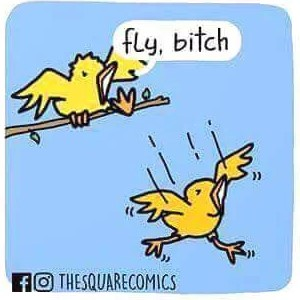
\includegraphics[width=0.5\textwidth]{images/fly.jpg}
\end{figure}



\end{document}